\chapter{Artificial Neural Network (ANN)}

\section{Perceptron \cite{wiki-perceptron}}\label{perceptron}

\begin{figure}[H]
    \centering
    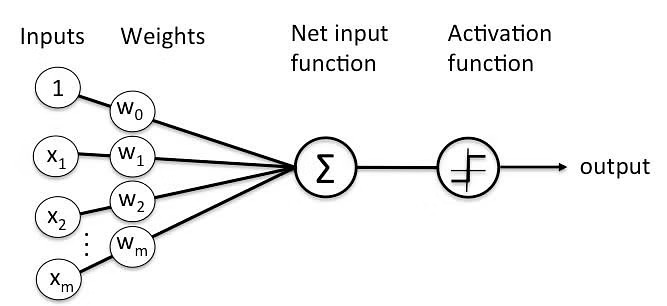
\includegraphics[height=3cm]{Pictures/deep_neural_networks/perceptron.jpg}
    \caption{Perceptron}
\end{figure}

In machine learning, the perceptron (or McCulloch–Pitts neuron) is an algorithm for supervised learning of binary classifiers. A binary classifier is a function which can decide whether or not an input, represented by a vector of numbers, belongs to some specific class. It is a type of linear classifier, i.e. a classification algorithm that makes its predictions based on a linear predictor function combining a set of weights with the feature vector.


\section{Artificial neuron \cite{wiki-Artificial_neuron}}\label{Artificial neuron}
\begin{table}[H]
    \begin{minipage}{0.45\textwidth}
        \begin{figure}[H]
            \centering
            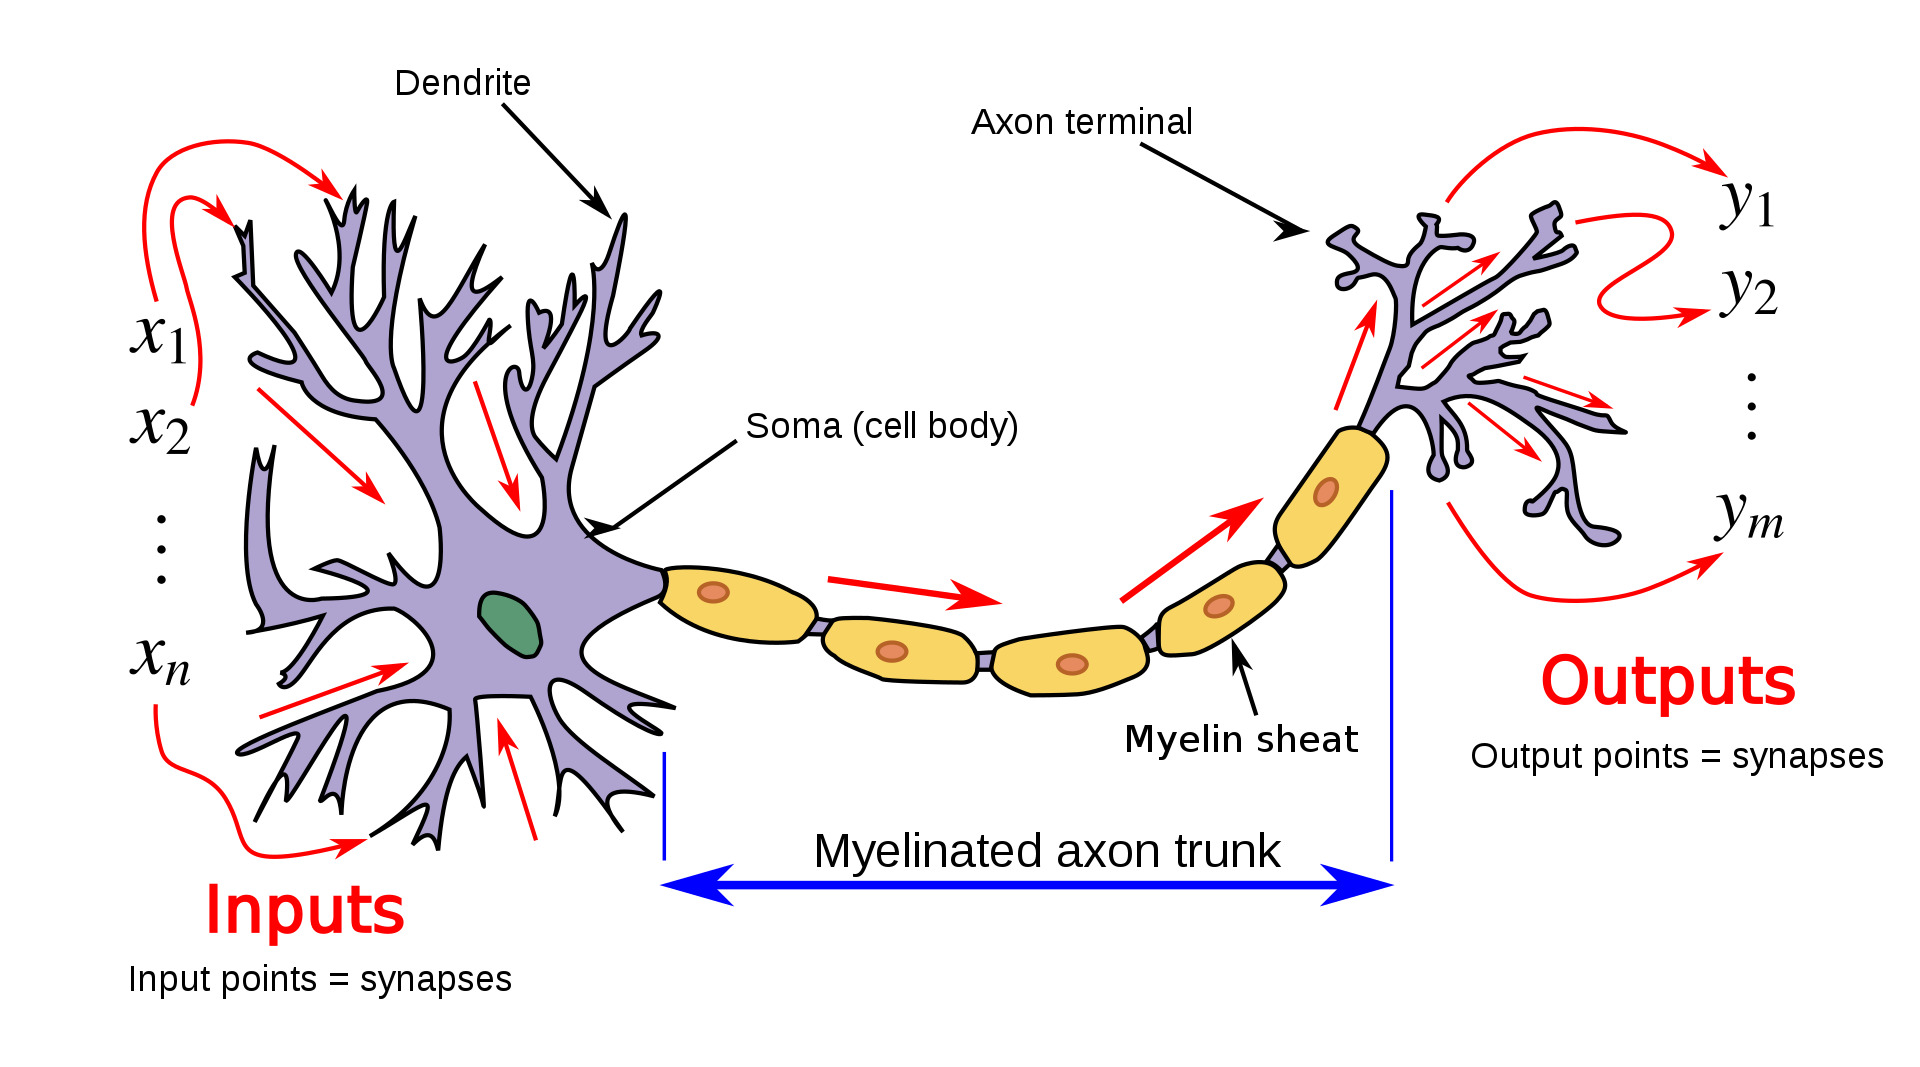
\includegraphics[height=4cm]{Pictures/deep_neural_networks/bio_neuron.jpg}
            \caption{ANN: Biological Neuron}
        \end{figure}
    \end{minipage}
    \hfill
    \begin{minipage}{0.45\textwidth}
        \begin{figure}[H]
            \centering
            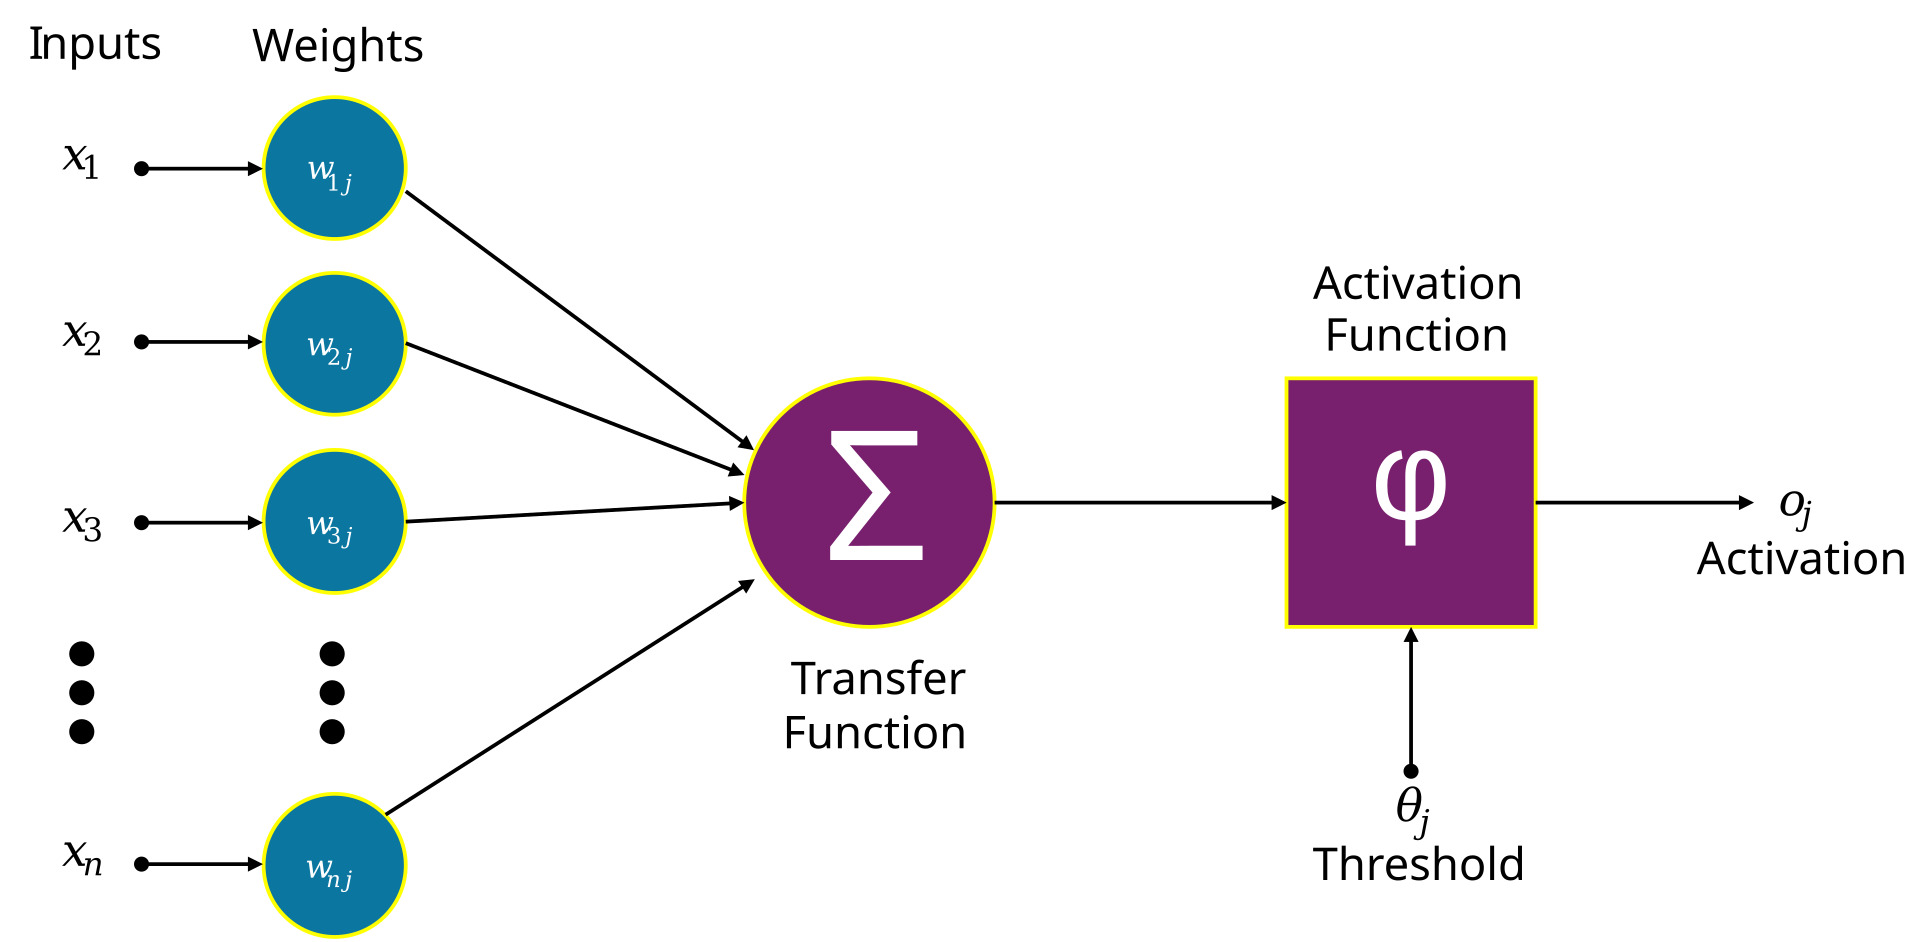
\includegraphics[height=4cm]{Pictures/deep_neural_networks/Artificial_neuron_structure.jpg}
            \caption{ANN: Artificial Neuron}
        \end{figure}
    \end{minipage}
\end{table}


An artificial neuron is a mathematical function conceived as a model of biological neurons in a neural network. Artificial neurons are the elementary units of artificial neural networks. The artificial neuron is a function that receives one or more inputs, applies weights to these inputs, and sums them to produce an output.


Usually, each input is separately weighted, and the sum is often added to a term known as a bias (loosely corresponding to the threshold potential), before being passed through a non-linear function known as an \textbf{activation function} or \textbf{transfer function}.

\[
     y_{k}=\varphi \left(\sum _{j=0}^{m}w_{kj}x_{j}\right)
\]


\section{Perceptron vs Artificial Neuron \cite{chatgpt}}
\begin{longtable}{| m{3cm} | m{6cm} | m{6cm} |}
    \caption{Perceptron vs Artificial Neuron} \\
    \hline
    \textbf{Feature} & \textbf{Perceptron} & \textbf{Neuron in a Neural Network} \\
    \hline
    \endfirsthead
    
    \hline
    \textbf{Feature} & \textbf{Perceptron} & \textbf{Neuron in a Neural Network} \\
    \hline
    \endhead
    
    \hline
    \endfoot
    
    \hline
    \endlastfoot
    
    \textbf{Definition} & A type of artificial neuron used in binary classifiers. & A general computational unit in a neural network. \\
    \hline
    \textbf{Activation Function} & Uses a step function (binary output: 0 or 1). & Uses various activation functions (e.g., ReLU, sigmoid, tanh). \\
    \hline
    \textbf{Complexity} & Simple and linear. & Can be complex and non-linear. \\
    \hline
    \textbf{Learning Rule} & Uses the perceptron learning rule. & Uses more advanced learning rules (e.g., backpropagation). \\
    \hline
    \textbf{Output} & Binary output (0 or 1). & Continuous output, depending on the activation function. \\
    \hline
    \textbf{Applications} & Suitable for linear classification tasks. & Suitable for both linear and non-linear tasks. \\
    \hline
    \textbf{Historical Context} & One of the earliest models of an artificial neuron, introduced by Frank Rosenblatt in 1958. & Evolved from the perceptron, used in modern deep learning. \\
    \hline
    \textbf{Layers} & Typically used in single-layer models. & Used in multiple layers (deep networks). \\
    \hline
    \textbf{Expressive Power} & Limited to linearly separable problems. & Can model complex relationships and patterns. \\
    \hline

\end{longtable}



\section{Activation Function \cite{wiki-Artificial_neuron, wiki-activation-fn}}
The activation function of a node in an artificial neural network is a function that calculates the output of the node based on its individual inputs and their weights. Nontrivial problems can be solved using only a few nodes if the activation function is nonlinear


\begin{itemize}
    \item  The transfer functions usually have a \textbf{sigmoid} shape, but they may also take the form of other non-linear functions, piecewise linear functions, or step functions.
    \item They are also often monotonically increasing, continuous, differentiable and bounded. 
    \item  Non-monotonic, unbounded and oscillating activation functions with multiple zeros that outperform sigmoidal and ReLU-like activation functions on many tasks have also been recently explored
\end{itemize}

See \ref{chapter: Activation Functions} for more details.


\section{Connectionism model \cite{wiki-Connectionism}}\label{Connectionism model}
Connectionism (coined by Edward Thorndike in the 1931) is the name of an approach to the study of human mental processes and cognition that utilizes mathematical models known as connectionist networks or artificial neural networks. Connectionism has had many 'waves' since its beginnings.

\section{Artificial Neural Network (ANN) \cite{wiki-ann}}\label{ann}
\begin{figure}[H]
    \centering
    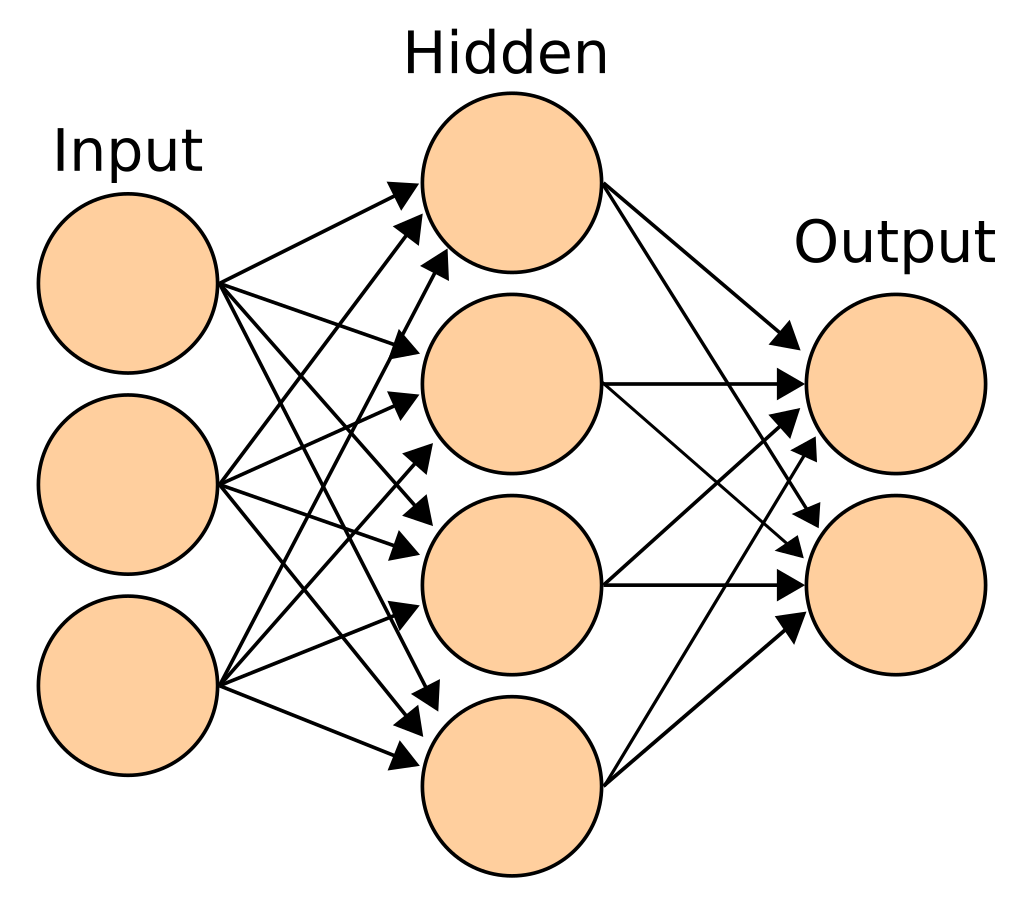
\includegraphics[height=4cm]{Pictures/deep_neural_networks/ann.png}
    \caption{Artificial Neural Network}
\end{figure}
A neural network (also artificial neural network or neural net, abbreviated ANN or NN) is a model inspired by the structure and function of biological neural networks in animal brains. An ANN consists of connected units or nodes called \textbf{artificial neurons}, which loosely model the neurons in a brain. These are connected by edges, which model the synapses in a brain. Each artificial neuron receives signals from connected neurons, then processes them and sends a signal to other connected neurons. The "signal" is a real number, and the output of each neuron is computed by some non-linear function of the sum of its inputs, called the \textbf{activation function}. The strength of the signal at each connection is determined by a weight, which adjusts during the learning process.

\section{Connectionism vs ANN \cite{chatgpt,arxiv-2405.04048}}\label{connectionism vs ann}
\begin{longtable}{|>{\raggedright\arraybackslash}p{3cm}|>{\raggedright\arraybackslash}p{6cm}|>{\raggedright\arraybackslash}p{6cm}|}
\caption{Connectionism vs ANN} \\
\hline
\textbf{Aspect} & \textbf{Connectionism} & \textbf{Artificial Neural Networks (ANNs)} \\
\hline
\endfirsthead
\hline
\textbf{Aspect} & \textbf{Connectionism} & \textbf{Artificial Neural Networks (ANNs)} \\
\hline
\endhead
\hline
\endfoot
\hline
\endlastfoot
\textbf{Definition} & Theoretical framework for understanding the mind using interconnected networks of simple units. & Computational models inspired by brain's neural networks, used in machine learning. \\
\hline
\textbf{Scope} & Broad approach to cognition and brain function. & Specific computational implementations within connectionism. \\
\hline
\textbf{Focus} & Understanding cognitive processes and brain function. & Practical machine learning applications. \\
\hline
\textbf{Origins} & Cognitive science and psychology. & Efforts to mimic brain function for computational purposes. \\
\hline
\textbf{Key Concepts} & Neural networks, learning, parallel distributed processing, emergent properties. & Architecture (layers), activation functions, training (e.g., backpropagation), types (e.g., CNNs, RNNs). \\
\hline
\textbf{Learning} & Adjusting connection strengths based on experience. & Training involves adjusting weights to minimize prediction errors. \\
\hline
\textbf{Information Processing} & Parallel and distributed. & Parallel and distributed, with specific architectures (e.g., feedforward, convolutional). \\
\hline
\textbf{Applications} & Understanding perception, memory, language; modeling psychological phenomena. & Image and speech recognition, natural language processing, autonomous vehicles, medical diagnosis, financial forecasting. \\
\hline
\textbf{Theoretical Foundation} & Provides conceptual framework for cognition and brain modeling. & Empirical support for connectionist theories, demonstrating learning and task performance. \\
\hline
\textbf{Practical Implementation} & Conceptual approach with some computational models. & Implementations used in AI and machine learning. \\
\hline
\end{longtable}

\begin{itemize}
    \item ANN is subset of Connectionism
\end{itemize}


\section{Perceptron Learning Algorithm \cite{medium-perceptron-learning-algorithm}}\label{Perceptron Learning Algorithm}

\begin{itemize}
    \item Goal is to find the w vector that can perfectly classify positive inputs and negative inputs in the data.
\end{itemize}

\begin{algorithm}[H]
    \caption{Perceptron Learning Algorithm}
    $P \gets$ inputs with label 1\;
    $N \gets$ inputs with label 0\;
    Initialize $\textbf{w}$ randomly\;
    \While{!convergence}{
        Pick random $x \in P \cup N$\;
        \If{$x \in P$ and $w \cdot x < 0$}{
            $w = w + x$\;
        }
        \If{$x \in N$ and $w \cdot x \ge 0$}{
            $w = w - x$\;
        }
    }
\end{algorithm}

Examples:\\
\begin{itemize}
    \item \url{https://www.geeksforgeeks.org/implementation-of-perceptron-algorithm-for-or-logic-gate-with-2-bit-binary-input/}
    \item \url{https://www.geeksforgeeks.org/implementation-of-perceptron-algorithm-for-and-logic-gate-with-2-bit-binary-input/}
    \item \url{https://www.geeksforgeeks.org/implementation-of-perceptron-algorithm-for-not-logic-gate/}
    \item \url{https://turcomat.org/index.php/turkbilmat/article/view/7786}
\end{itemize}



\section{Multilayer Perceptron (MLP) \cite{wiki-Multilayer_perceptron}}\label{Multilayer_perceptron}
A multilayer perceptron (MLP) is a name for a modern feedforward artificial neural network, consisting of fully connected neurons with a nonlinear activation function, organized in at least three layers, notable for being able to distinguish data that is not linearly separable. \\
Modern feedforward networks are trained using the backpropagation method and are colloquially referred to as the "vanilla" neural networks.\\
MLPs grew out of an effort to improve single-layer perceptrons, which could only distinguish linearly separable data. A perceptron traditionally used a Heaviside step function as its nonlinear activation function. However, the backpropagation algorithm requires that modern MLPs use continuous activation functions such as sigmoid or ReLU.

\section{Multilayer Perceptron (MLP) vs Artificial Neural Network (ANN)}\label{mlp vs ann}
\begin{longtable}{|>{\raggedright}m{4cm}|>{\raggedright}m{5cm}|>{\raggedright\arraybackslash}m{5cm}|}
    \caption{Multilayer Perceptron (MLP) vs Artificial Neural Network (ANN)}\\
    \hline
    \textbf{Feature} & \textbf{MLP (Multilayer Perceptron)} & \textbf{ANN (Artificial Neural Network)} \\
    \hline
    \endfirsthead
    \hline
    \textbf{Feature} & \textbf{Multilayer Perceptron (MLP)} & \textbf{Artificial Neural Network (ANN)} \\
    \hline
    \endhead
    \endfoot
    \hline
    \endlastfoot
    \textbf{Definition} & A type of ANN with multiple layers & A broad category of machine learning models inspired by the human brain \\
    \hline
    \textbf{Structure} & Consists of input, hidden, and output layers & Can have various structures, including MLP, CNN, RNN, etc. \\
    \hline
    \textbf{Layers} & Always has at least one hidden layer & Can have any number of layers and types \\
    \hline
    \textbf{Neurons} & Fully connected layers of neurons & Can include different types of neurons (e.g., convolutional, recurrent) \\
    \hline
    \textbf{Training} & Typically trained with backpropagation & Can be trained with various algorithms depending on the type \\
    \hline
    \textbf{Usage} & Commonly used for classification and regression tasks & Used for a wide range of tasks including image recognition, natural language processing, etc. \\
    \hline
    \textbf{Complexity} & Generally less complex compared to other ANNs like CNNs and RNNs & Can range from simple to highly complex models \\
    \hline
    \textbf{Flexibility} & Less flexible compared to other ANN architectures & Highly flexible with many architectures available \\
\end{longtable}

\begin{itemize}
    \item MLP is a specific type of ANN, meaning all MLPs are ANNs, but not all ANNs are MLPs.
\end{itemize}


\section{Width \& Depth of ANN/ MLP \cite{arxiv-2010.15327}}




























































































